\chapter{Concept}
\textit{In this chapter, I will discuss the concept that addressed the topics  of  stress management requirement engineering and design approach. I have  chosen requirement engineering that  assisted  us  to design a system for stress management at  the  workplace  in  particular  for People with stress disability. To have  a clear understanding of the requirement, I have chosen the design process. It organizes my ideas and refines potential solutions to engineering challenges. Afterwards, a  system is designed which is satisfy my goal.}
\vspace{5mm}

Stress has recently overtaken the common cold as the most common cause of sick leave in many European countries and is a major cause of concern for companies worldwide. Why then do most of the 'Coping with Stress' texts to be found in bookshops consider this a problem only to be tackled by the Individual? Strategic Stress Management is different, it shows how companies can boost performance by adopting integrated organizational strategies to identify and reduce stress in their employees. Including practical advice on how to conduct a stress audit and how to target stress 'hot spots' with an organization, Strategic Stress Management provides a fresh strategic model for the manager which concern with the negative effects stress can have both on company performance and the quality of life of individuals at work. This is the latest book from best-selling stress management author, Cary Cooper, and will be eagerly awaited by HR Directors, Organizational Consultants. Occupational Psychologists, Managing Directors and all managers who wish to work with healthy, stable and productive staff.

\section{Requirement Engineering}
The ultimate aim of writing a problem statement is to turn a common problem into a targeted, well-defined problem that can be solved through a requirement engineering process. It indicates the project's purpose. \citep{K.AduMichael2014InadequateStudy.}

\begin{figure}[ht!]
\centering
\smartdiagramset{
planet color=orange!60,
distance planet-satellite=4cm,
planet text width=2.5cm,
satellite text width=2.7cm,
}
\smartdiagram[connected constellation diagram]{
    Requirement Engineering,
    Feasibility\\study,
    Analysis,
    Definition,
    Documentation
}
\captionof{figure}{Requirement Engineering Steps}
  \label{fig:RE}
\end{figure}

It is a process of gathering and defining service provided by the system.My requirements Engineering Process consists of the following main activities: shows in the figure:\ref{fig:RE}

\begin{enumerate}
    \item  Feasibility study : find out the current user need and budget.
    \item Requirement analysis: what the stakeholders required from the system.
    \item Requirement definition: defined the requirements in the form of understandable to the customer.
    \item Requirement document: official statement define both, definition and specification.
\end{enumerate}

The current research aimed to explore the effectiveness of a system that promotes behavioural change for stress-related issues in terms of the acceptability, usefulness and possible effects of the program. Furthermore, the aim is also to study how appropriate and realistic the process and resource management of the study would be for a randomized controlled trial. \citep{Eklund2018EvaluationStudy}

When conducting a feasibility investigation, the important parameters for a planned, randomized controlled trial can be identified, adjusted, and further developed to improve the chances of success in a larger, more costly study. Feasibility studies can help identify what needs to be changed in terms of action and research methodology. 

I asked only one participant for my study. It is impossible to learn everything about participants within the limited time available for interviews and observation, so try to ask the most advantageous questions and notice the most relevant behaviour.To determine what information is most needed, consider my knowledge gaps, what details would best suit my design decisions, and what would give me a common frame of reference regarding the needs and goals of the participants. That's why one is enough for my study.
 
 This study for a specific target group and customized system based on user behaviour. My participant is a perfect match for this study. By capturing the essence of my perspectives from asking the right questions, I will be able to create a persona that brings their voice into the conversation. I will get the required data to create a persona from the right kind of information is the best proxy. I have done a personal interview to conduct feasibility studies based on a random set of questionnaires. I set this questionnaire based on \cite{Michie2002CausesWork.} stress table. The participant could answer freely based on their own experience. Following table:\ref{tab:feasibility} describe the result of my interview. 

\begin{table}[ht!]
\centering
\begin{tabular}{|l|l|}
\hline
\textbf{Questions} & \textbf{Answers} \\ 
\hline
Do you feel stress in Working Place? & Yes \\ 
\hline
\begin{tabular}[c]{@{}l@{}}Can you describe a time when your \\ stress resulted in making errors at work?\end{tabular} & Evening \\ \hline
What are the signs of your stress in the workplace? & Can not communicate with others  \\ \hline
How common is stress in the workplace? & Almost Everyday \\ \hline
\begin{tabular}[c]{@{}l@{}}What’s the most stressful situation \\ you’ve faced at work so far? How did you handle it?\end{tabular} & In meeting \& leave the place \\ \hline
When you feel stress what happened in physically?? & Feeling imbalanced  \\ \hline
\end{tabular}
\caption{Feasibility Study Questionnaires \& Answers }
\label{tab:feasibility}
\end{table}

Considering the program's acceptability, the findings for the statements evaluating the opinions and experiences of the participants concerning the content, tailoring, input, performing an own behavioural analysis, setting goals, graphic and pedagogical design, and how the knowledge is summarized in Table: \ref{tab:feasibility}

As a result of my questionnaires, To enhance flexibility, participants suggested that stress Management should be delivered as a mobile application with IoT devices. Stress Management structure forces the user to go through all the assignments in a predetermined order, and this is perceived as a barrier for using. The participant with low-stress levels expressed that for a person with a low-stress level, it was difficult to stay motivated to go through such an extensive program.

In the next section, I am going to develop a design approach.

\section{Design Approach}
Providing this real information about users will enable agile, progressive or repetitive progress along the development process. In this regard, personas, which are commonly used in user-centred design and human-computer interaction activities, are not only a suitable method for the adequate documentation of users’ attributes but also a tool for empathizing with users’ aims and needs. Personas can be used throughout the entire development process and in addition to user-based design tasks by the development team for requirement engineering activities.

The integration of personas, as a kind of user description, in the requirements engineering activities, improves two aspects of the development: (1) consideration of multi-faceted user needs in the early stages of development when practical main decisions are taken; (2) continuous integration, testing and revision of user requirements for evaluation of existing prototypes and intermediates.\citep{Mayas2016PersonasChallenges}

\subsection{Persona analysis}
% https://app.milanote.com/1IW8dZ1W4EN68B/jan
\begin{figure}[hbt!] 
  \centering
  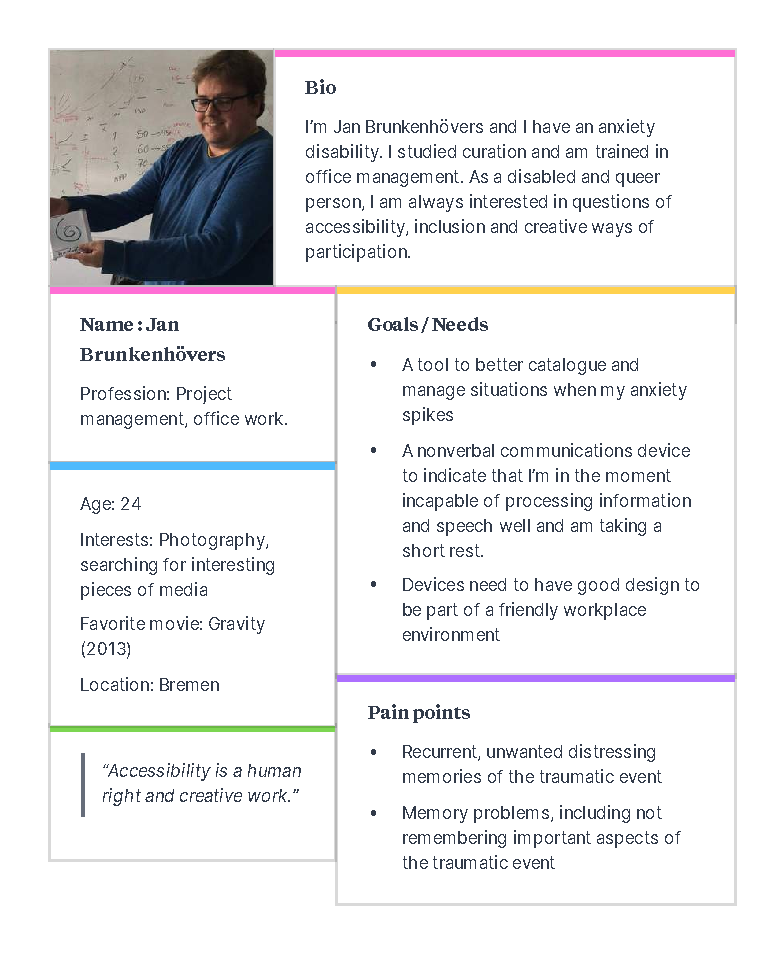
\includegraphics[width=1.05\linewidth]{chap3/image/persona_jans.pdf}
  \caption[Persona Analysis ]{Persona Analysis.\index{Hasnain}}
  \label{fig:Persona_Analysis}
\end{figure}


In Figure \ref{fig:Persona_Analysis} you can see the persona analysis dashboard which has made for the design more specific application for the user.

The result of Persona Analysis will be determined based on the following data from the user:

\begin{itemize}
    \item User Name : Jan Brunkenhövers
    \item Audience segment: Workplace accessibility for anxiety related disability
\end{itemize}
\subsubsection*{Bio}
    "I’m Jan Brunkenhövers and I have an anxiety disability. I studied curation and am trained in office management. As a disabled and queer person, I am always interested in questions of accessibility, inclusion and creative ways of participation."
\subsubsection*{Personal Information}
\begin{itemize}
\item Age: not mentioned
\item male
\item Interests: Photography, searching for interesting pieces of media.
\item Favorite movie: Gravity (2013)
\item Location: Bremen 
\end{itemize}
\subsubsection*{Goals and Needs}
\begin{itemize}
    \item A tool to better catalogue and manage situations when my anxiety spikes
    \item A nonverbal communications device to indicate that I’m in the moment incapable of processing information and speech well and am taking a short rest.
    \item Devices need to have a good design to be part of a friendly workplace environment   
\end{itemize}
% https://app.milanote.com/1IW8dZ1W4EN68B/jan

\subsubsection*{Pain points}
\begin{itemize}
    \item Recurrent, unwanted distressing memories of the traumatic event
    \item Memory problems, including not remembering important aspects of the traumatic event
\end{itemize}

\subsubsection{Analysis Outcome}\label{Persona Analysis Outcome}
\begin{figure}[hbt!] 
  \centering
  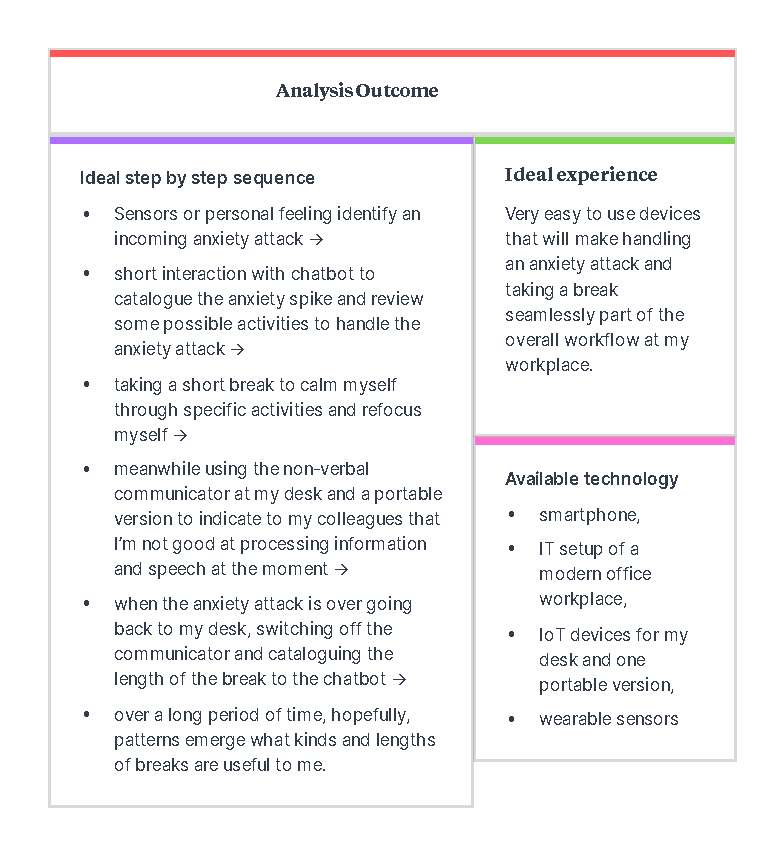
\includegraphics[width=1.04\linewidth]{chap3/image/persona_jans2.pdf}
  \caption[Persona Analysis outcome ]{Persona Analysis Outcome.\index{Hasnain}}
  \label{fig:Persona_Analysis2}
\end{figure}
\subsubsection*{Ideal step by step sequence}
\begin{itemize}
    \item Sensors or personal feeling identify an incoming anxiety attack 
    \item short interaction with the chatbot to catalogue the anxiety spike and review some possible activities to handle the anxiety attack 
    \item taking a short break to calm me through specific activities and refocus myself 
    \item meanwhile using the non-verbal communicator at my desk and a portable version to indicate to my colleagues that I’m not good at processing information and speech at the moment 
    \item when the anxiety attack is over going back to my desk, switching off the communicator and cataloguing the length of the break to the chatbot 
    \item over a long period, hopefully, patterns emerge what kinds and lengths of breaks are useful to me.
\end{itemize}
\subsubsection*{Available technology}
\begin{itemize}
    \item Smartphone
    \item IT setup of a modern office workplace
    \item IoT devices for my desk and one portable version
    \item wearable sensors
    \item Web applications and software.
\end{itemize}
\begin{figure}[ht] 
  \centering
  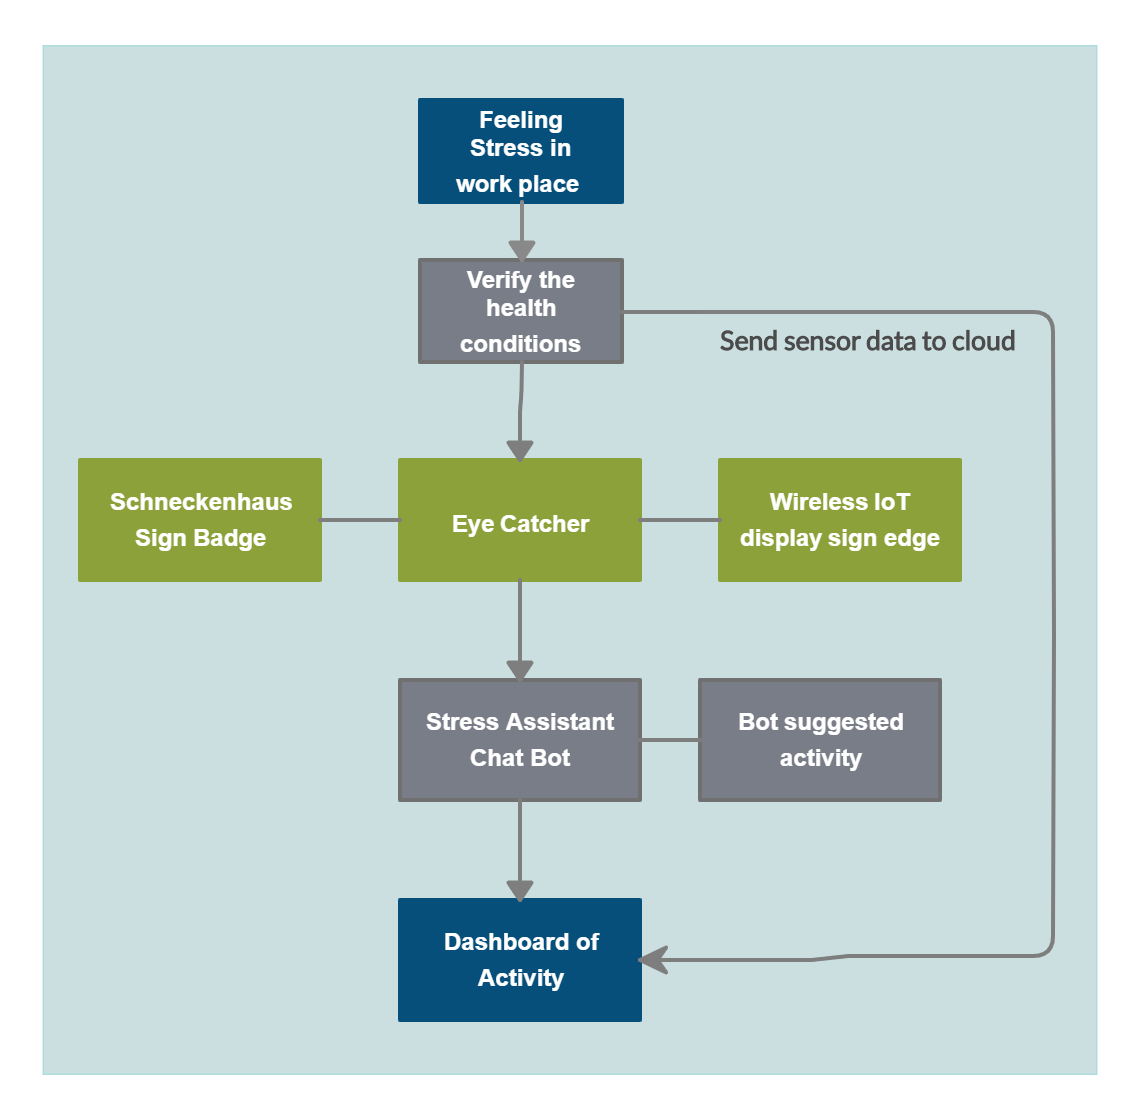
\includegraphics[width=1\textwidth]{chap4/block1.png} %https://app.creately.com/diagram/FLSbOaB2Ejl/edit
  \caption[Stress management System Block Diagram]{Stress management System Block Diagram \index{Hasnain}}
  \label{fig:system_block}
\end{figure}
\subsubsection*{Ideal experience}
Jan said his experience after analysis "Very easy to use devices that will make handling an anxiety attack and taking a break seamlessly part of the overall workflow at my workplace."

based on persona analysis I designed and make a prototype of the application which explain in the next section.

\subsection{Use case-driven system block diagram}
In figure \ref{fig:system_block}, I generate a system block diagram to approach it for implementation cases that I receive from persona analysis. This system block diagram is a high-level system modularization that divides the system as a whole into maximally decoupled sub-systems. It helps one to imagine the system as large interacting components, which can be independently conceptualized and created.


\section{Prototyping of the Application}

After the persona analysis and block diagram of the application, before start implementing and developing it, prototyping has been used as the first step in the design process.

Prototyping is not just about designing a user interface's "feel." It's also about prototyping — deciding how the \acs{UI} should work, and reacting to user input. That is why the design of interaction and the use of cases function together so well, especially when combined with people.\citep{Stephens2006PersonaAnalysis}

\subsection{Paper Prototyping}

\begin{figure}[hbt!] 
  \centering
  \subbottom[Sketch welcome page]{
\includegraphics[width=0.45\textwidth]{chap3/image/sk1.jpg}}\qquad
    \subbottom[Sketch Options]{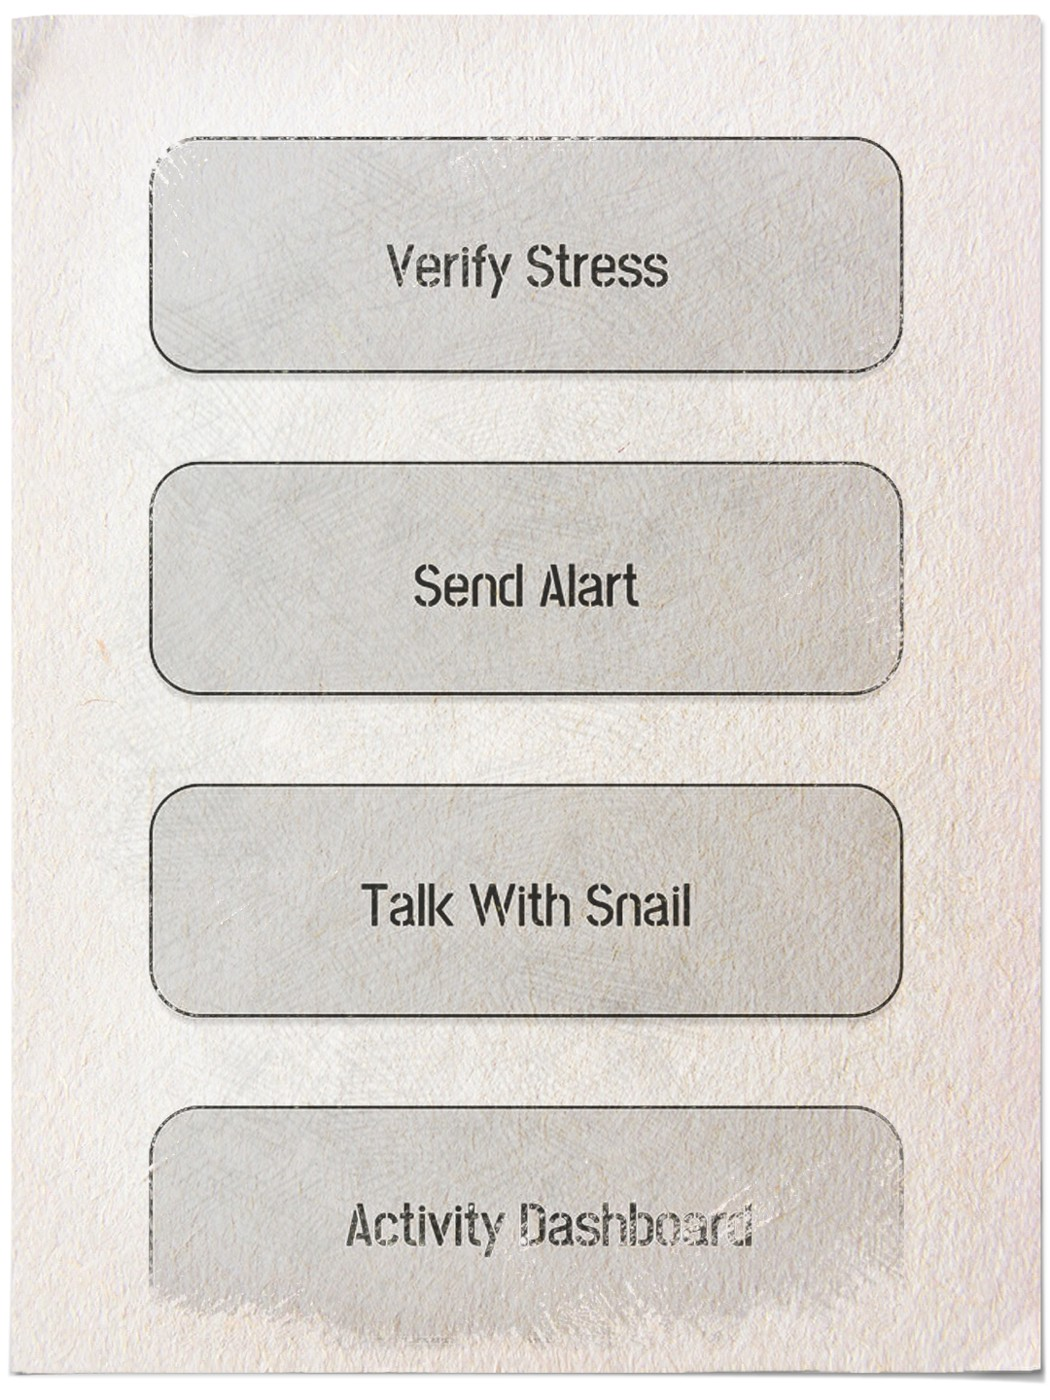
\includegraphics[width=0.45\textwidth]{chap3/image/sk2.jpg}}%
  \caption[Paper prototype sketch ]{Paper prototype sketch .\index{Hasnain}}
  \label{fig:Paper_proto}
\end{figure}
Paper prototyping which is also called as offline prototyping is the fastest way to get the straight feedback from the user in the initial stages of the design process and it also makes the discussion easier between the developers and other stakeholders of the app. The easiest ways to create paper prototypes include the use of cardboard, paper, pens and sticky notes.\citep{Bansemir2014ExperienceVisualizations}

The sketches made in paper prototypes create a mutual understanding of the interface of the application between the different stakeholders of the app which further positively affects the development process. It is being said that user and developers find sketches easier to understand the lengthy written documentation. Sketches which are being used in the process of paper prototyping presents the initial ideas of the app and build the foundation of discussions for the further iteration stages\citep{Bansemir2014ExperienceVisualizations}.

I sketch an example system (see In Figure \ref{fig:Paper_proto})  which has been made for the first look of workplace stress management system. This screen is normally referred to as virtual accessibility assistance or welcome screen. you can see a rough sketch of the buttons which I have used for accessing different functionality. 

One of the great things about paper prototypes is the way I can come up with all kinds of creative ways of simulating visual effects or interactions.

I plan to conduct testing sessions with a paper prototype and use two roles for each testing session:
\begin{itemize}
    \item Facilitator (presenter). A person who instructs and interacts with the test participants.
    \item 'Human-computer' This person remains silent during the session and is responsible for changing screens or screen statements whenever the participant of the test interacts with a prototype.
\end{itemize}

I give the name "Schneckenhaus" to this system. Schneckenhaus is the German name of an English snail shell. I used this \textbf{Schneckenhaus} as a metaphor of our stress management system. Snail shell thinking slow and it also has brain function problems which are similar to a human organ. It is a mental health symbol for struggling with memory and dementia as neurology challenges \citep{Zachos2018TraumaResearch}.

In Figure \ref{fig:Poster}, is an example of the testing sessions with a paper prototype which has been made for simulating visual effects of workplace stress management system.

\begin{figure}[hbt!] 
  \centering
  \subbottom[Schneckenhaus Sign Badge]{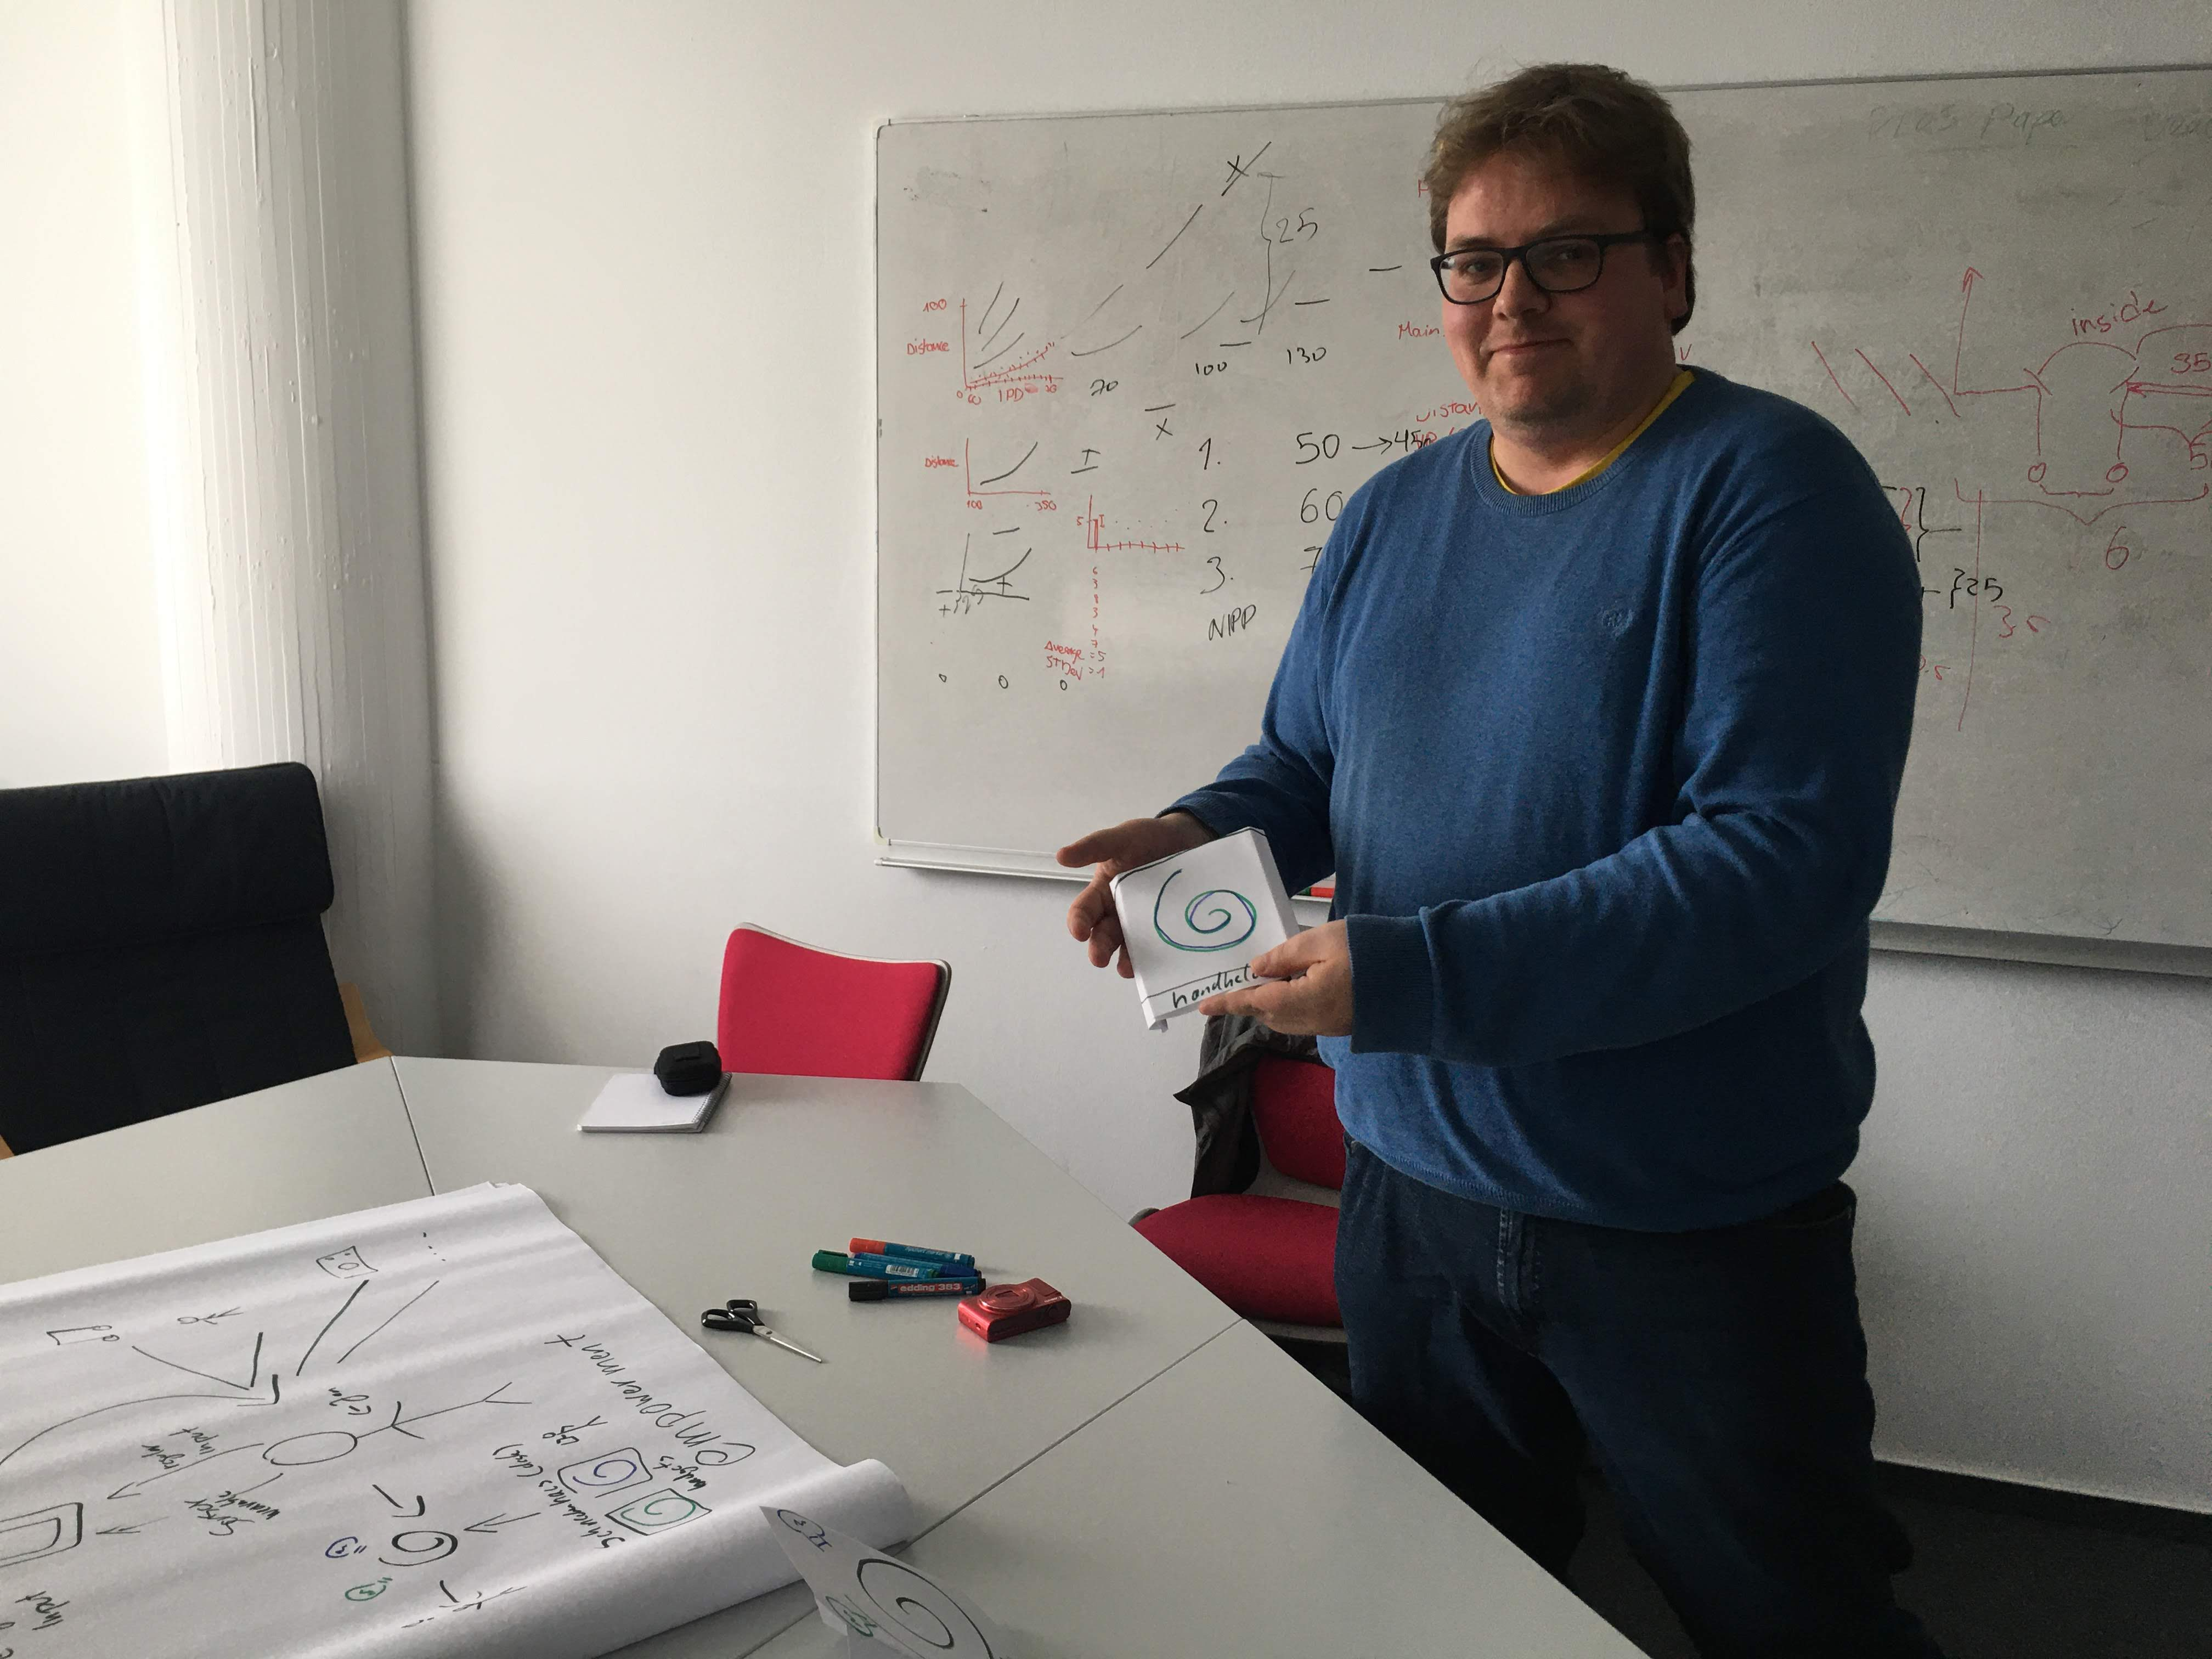
\includegraphics[width=0.45\textwidth]{chap3/image/jan1.JPG}}\qquad
    \subbottom[System Sketch ]{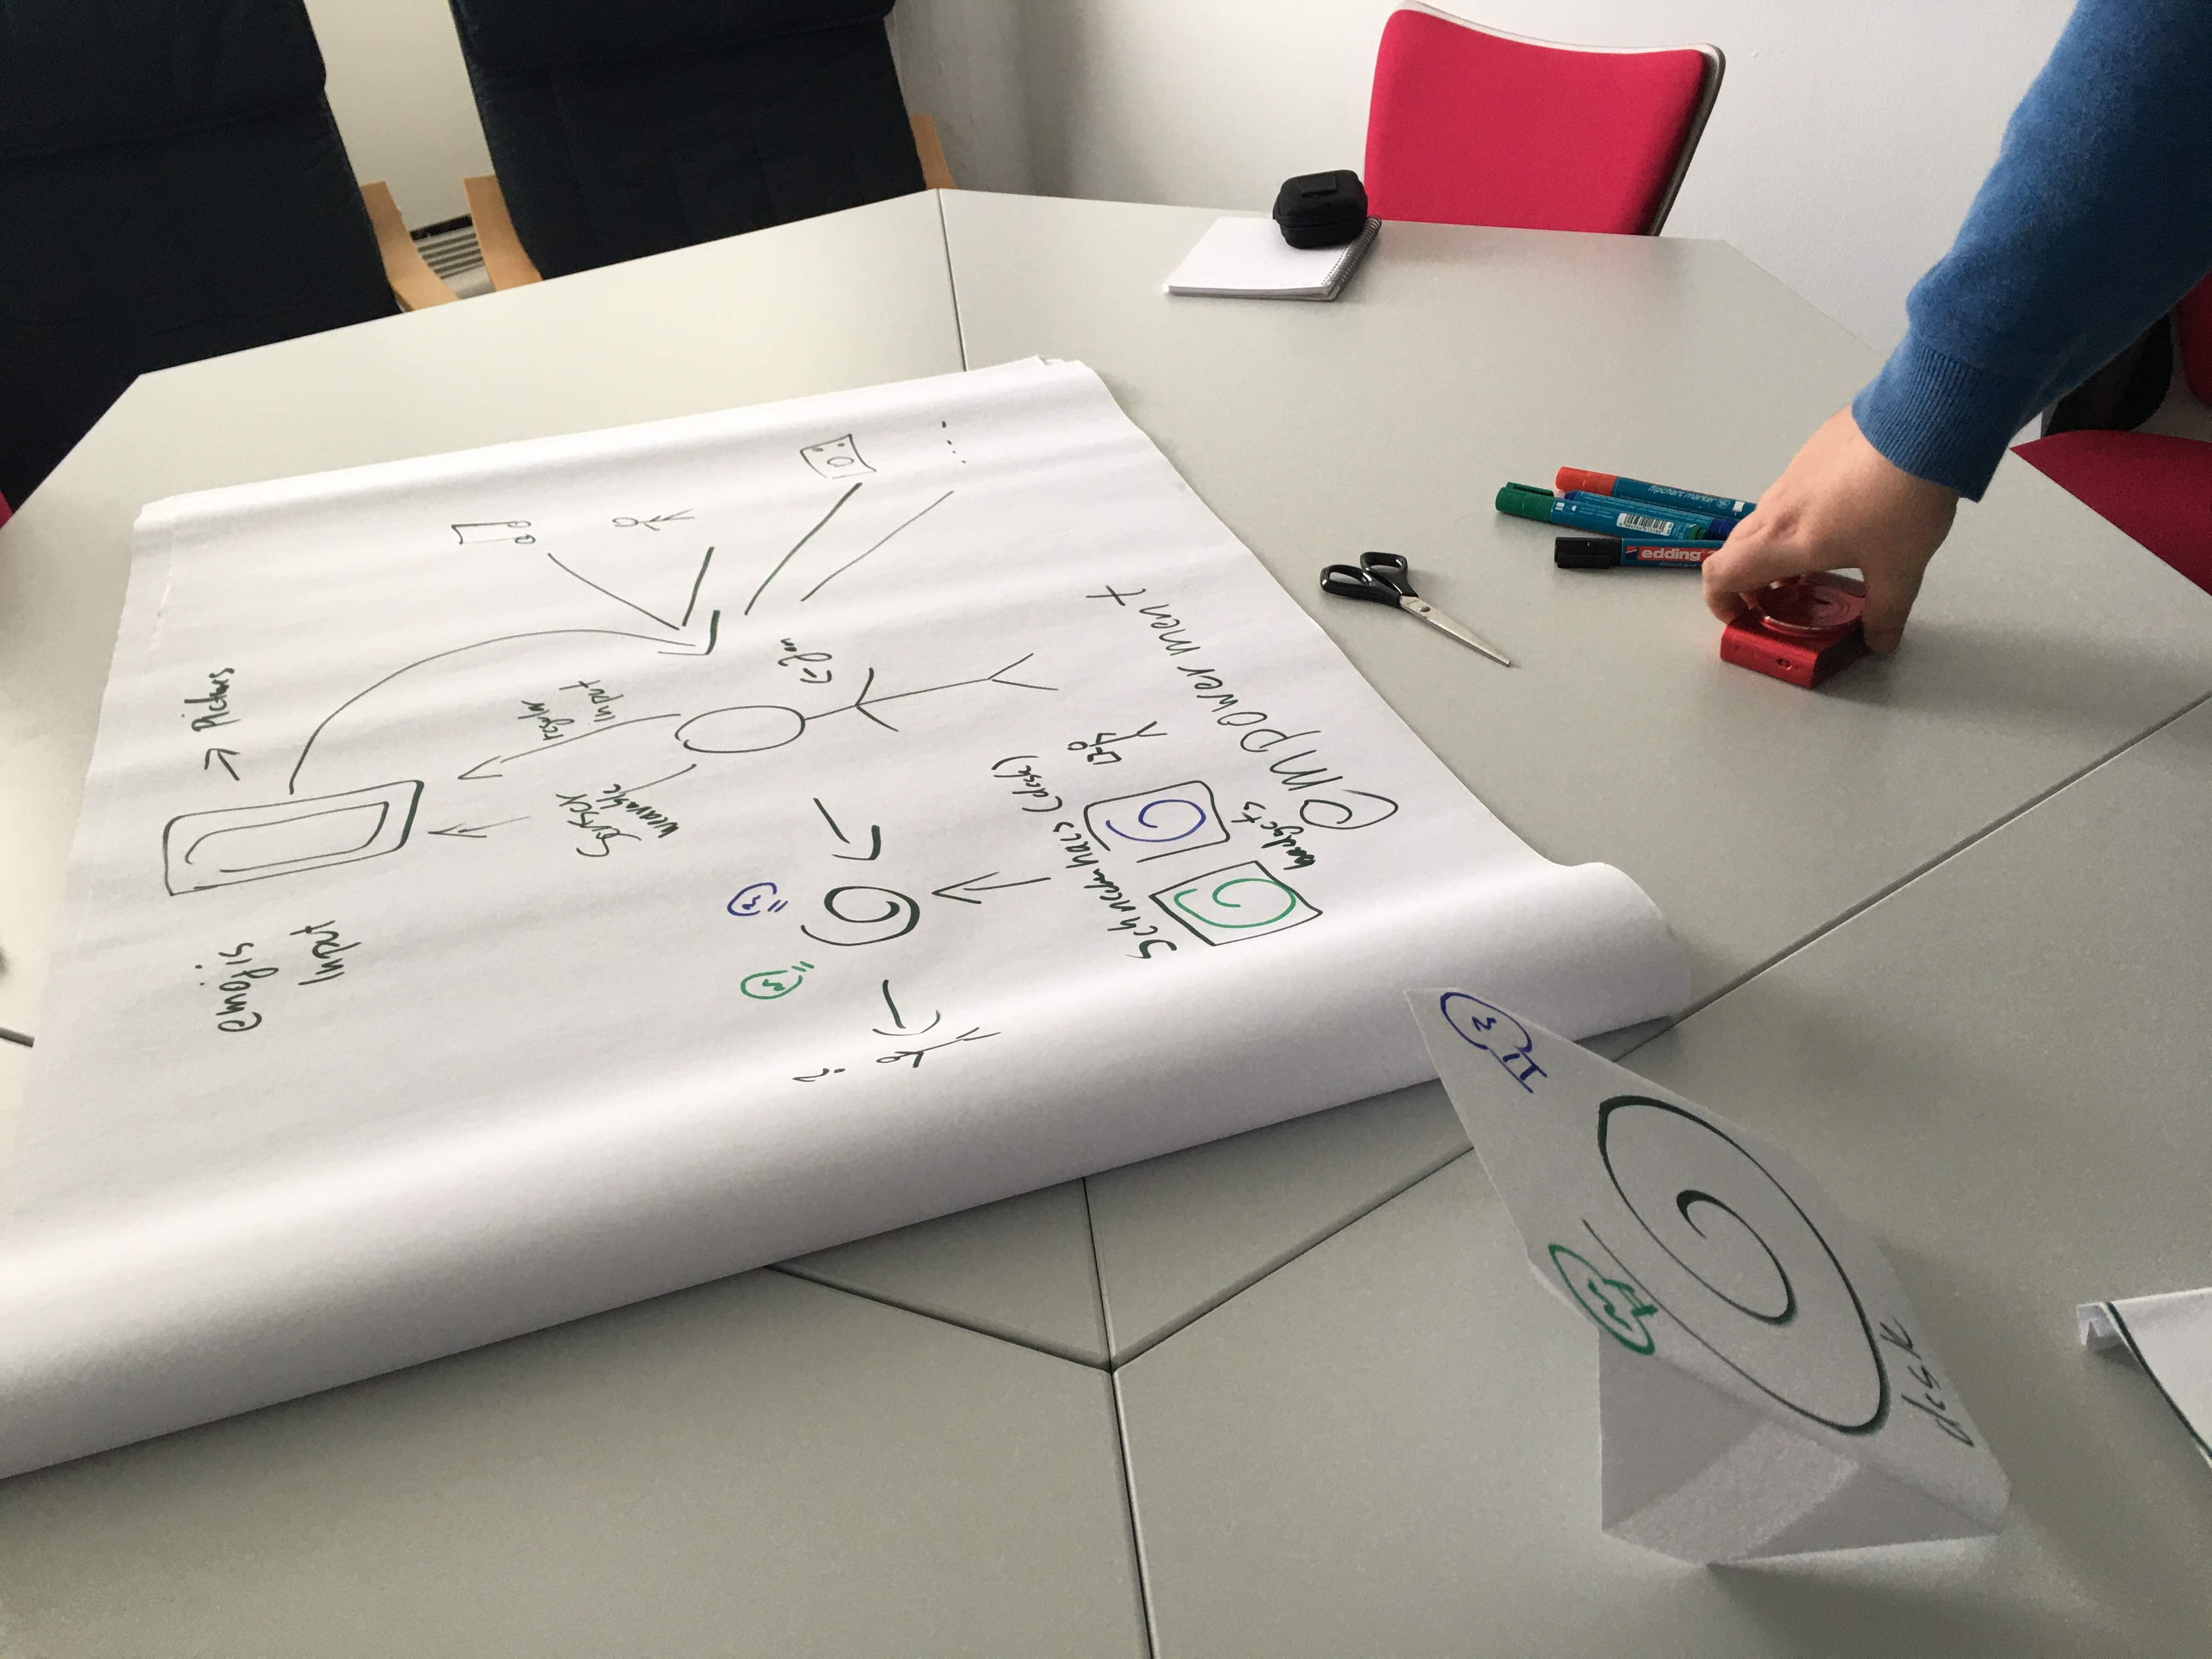
\includegraphics[width=0.45\textwidth]{chap3/image/jan2.JPG}}\qquad
    \subbottom[Perform Activity]{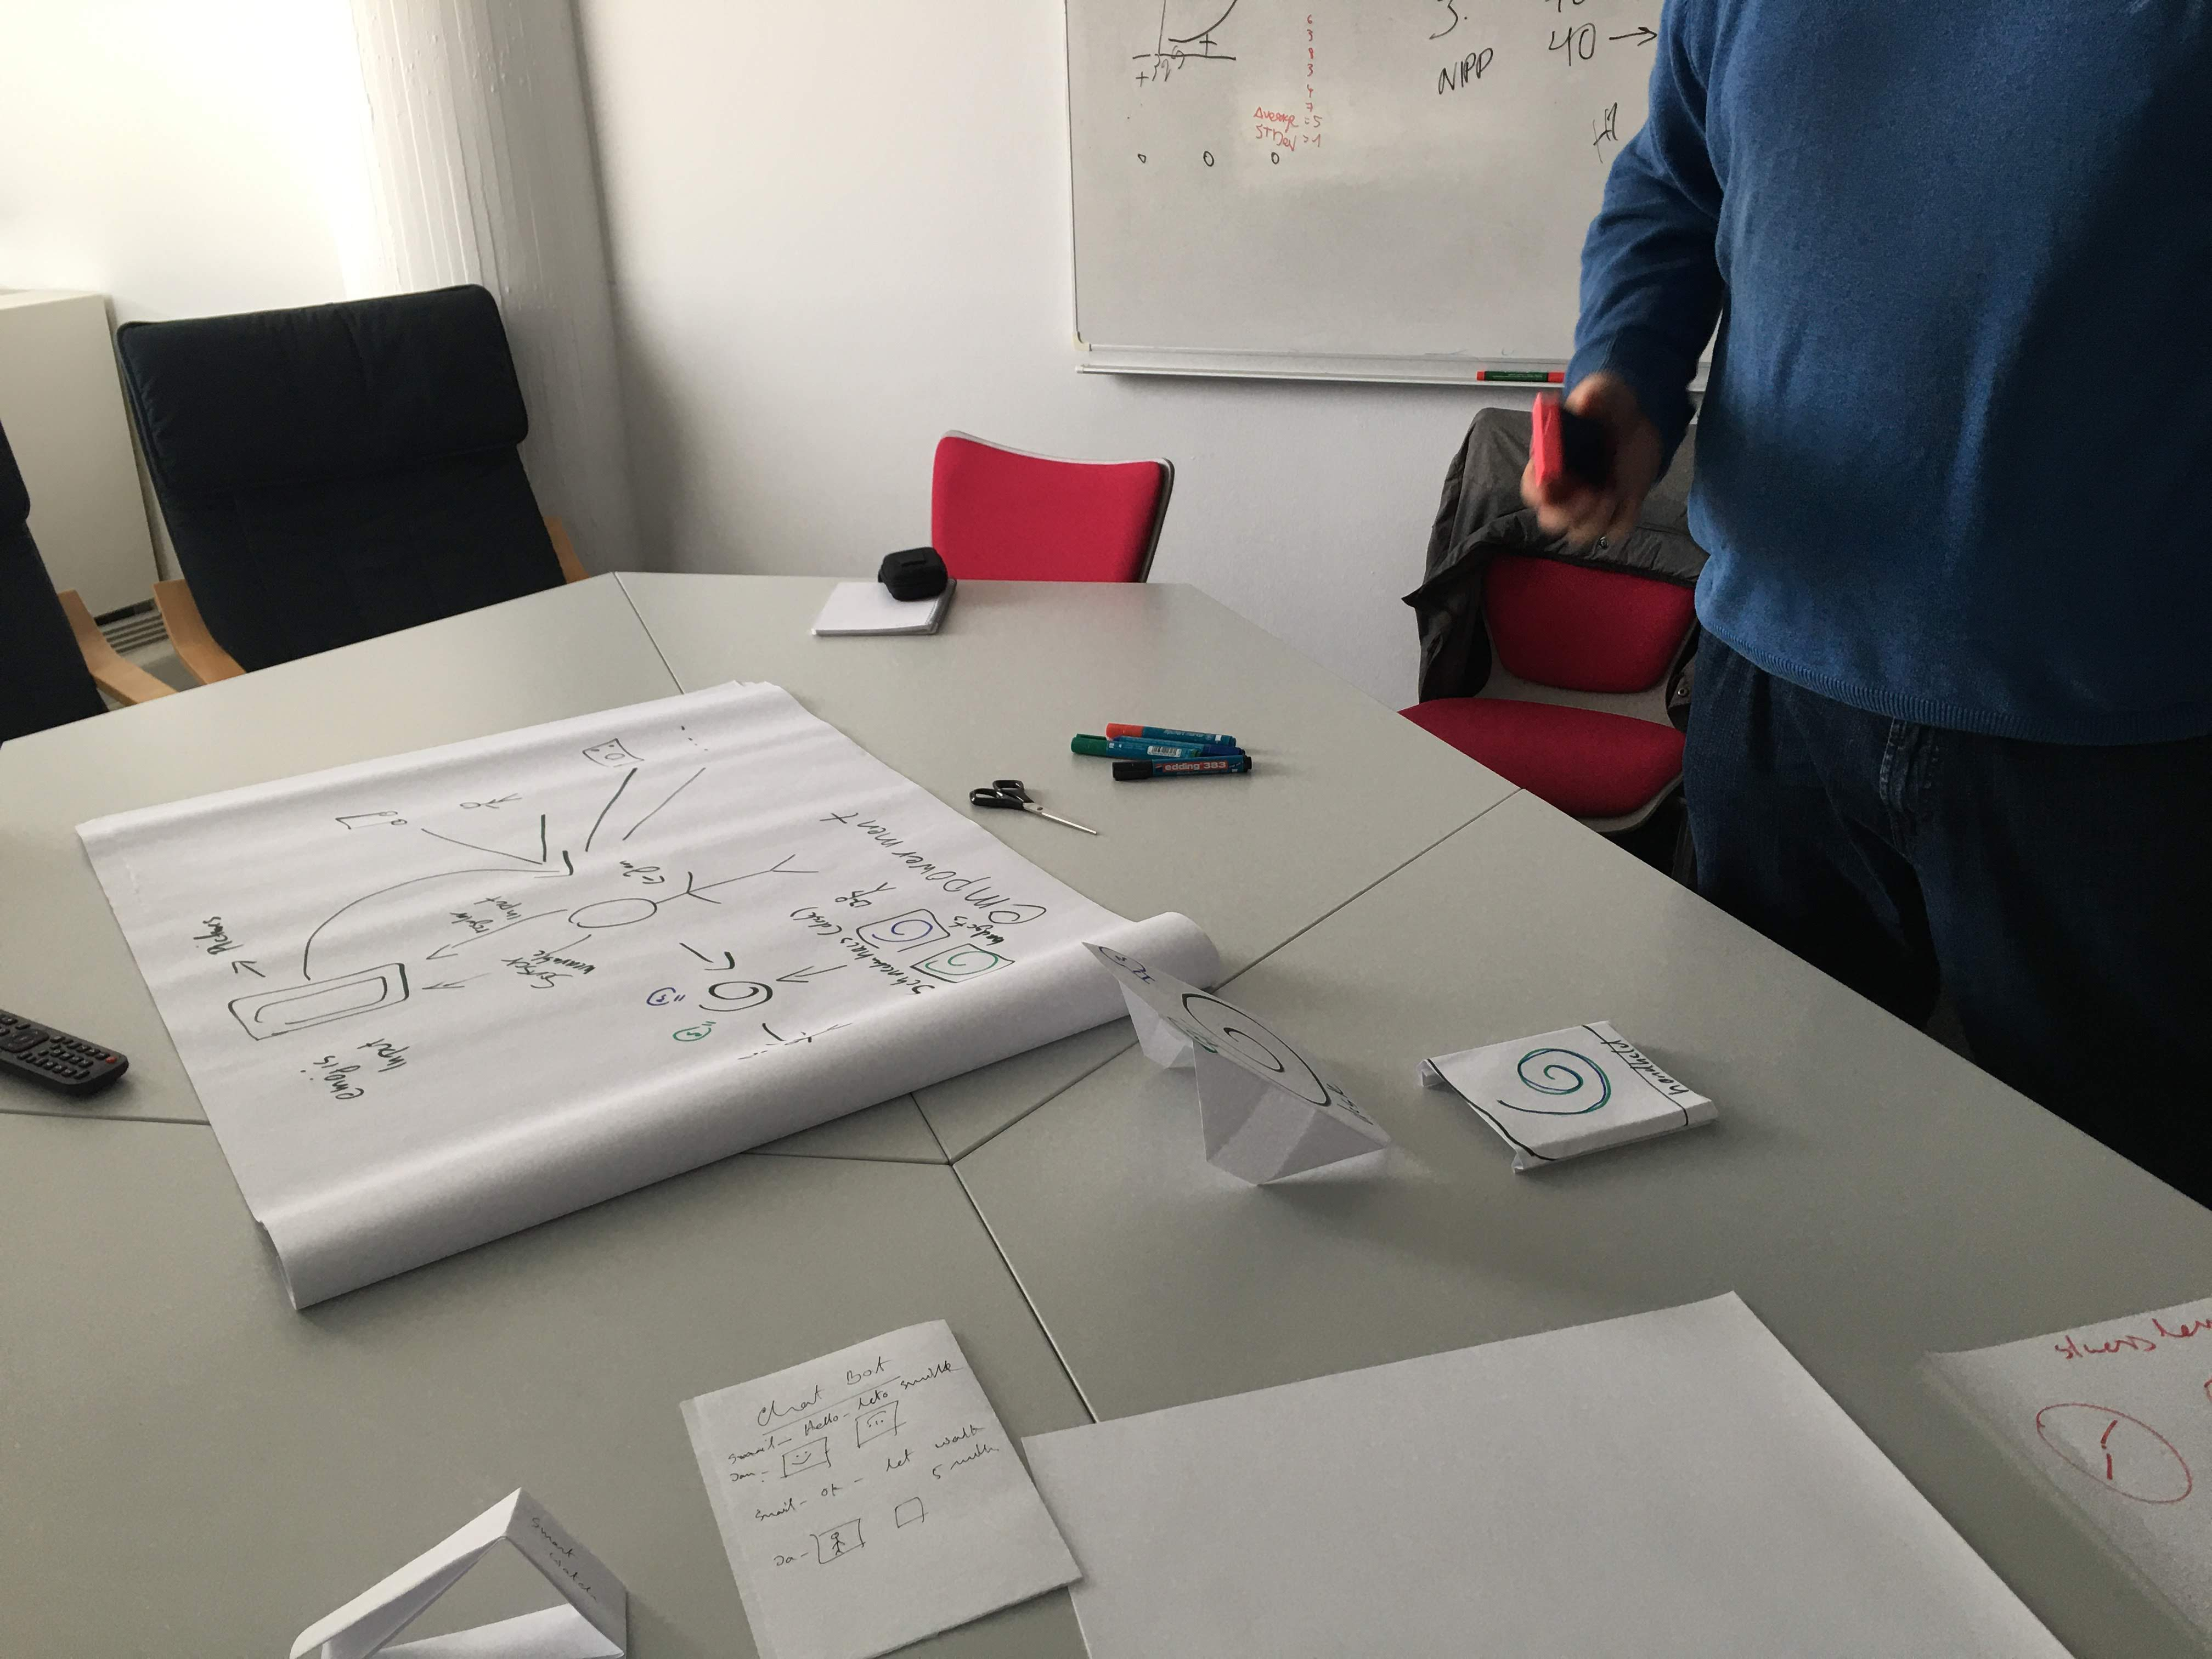
\includegraphics[width=0.45\textwidth]{chap3/image/jan3.JPG}}%
  \caption[Paper prototype Test session ]{Paper prototype Test session .\index{Hasnain}}
  \label{fig:Poster}
\end{figure}


\subsection*{Instruction for Paper prototype}

Instruct the participant to follow below mention instruction to start paper prototyping:

Imagine you are in your workplace and participating in a serious company meeting. Suddenly you feel stress overflowed. then check the following status and do activity accordingly.
\begin{itemize}
    \item For verify stress level open Schneckenhaus app. 
    \item click verify option to check stress status using a smartwatch, Spo2 sensors
    \item After verifying the stress level Turn on eye-catcher, send a message to wireless display, wear a badge.
    \item then talk with Snail chatbot. This bot will instruct user few activities based on current stress level and user conversation flow.
    \item Lastly user can check own activity on activity analytic dashboard.
\end{itemize}

\subsection*{Findings of Paper prototype} \label{Findings of Paper prototype}

Admittedly, in the beginning, this paper prototype test was rather giggly to me. Working with paper, scissors and glue-like some 5-year old kids in kindergarten. But soon I became more serious as meaningful GUI design discussions picked up. And after the first test run, I had missed quite a few interaction paths when discovered, realized that this paper prototyping technique was quite interesting and useful for my thesis.

An additional advantage of using this technique is that the impact of the GUI's eventual graphic design is a total non-factor. This allows testers to me only with functionality, without distractions. And then, when I later apply the graphic design, I have a wealth of information about the user interaction and how I need to direct it.

The screenshots of this application which has been planned and designed in the prototyping phase can be seen in Appendix A.


To sum up; this chapter has been discussed the concept and prototyping chosen to perform this study. I have addressed the requirement engineering and persona analysis considerations and also gave reasons as to why I chose this concept. The next chapter of my thesis will be present The Schneckenhaus system development. 


%\enlargethispage{\baselineskip} % so you do not get a single line in another page